\def\layersep{3cm}
\def\outsep{0.7cm}
\def\dy{1.5}

\begin{tikzpicture}[->, >=stealth, shorten >= 0pt, draw=black!50, node distance=\layersep, font=\sffamily]
    \tikzstyle{node}=[circle,fill=black,minimum size=2pt,inner sep=0pt]
    \tikzstyle{block}=[draw=black,rectangle,fill=none,minimum size=1cm, inner sep=0pt]
    \tikzstyle{annot} = []

	\node[node] (xc) at (0, 0 cm) {};
    \node[block, minimum size=2cm, text width=2cm, align=center] (RNN) at (1*\layersep, 0 cm) {Recurrent Neural Network};
	\node[block, text width=2cm, align=center] (O1) at (2*\layersep, \dy cm) {Probability of begin `A'};
	\node[block, text width=2cm, align=center] (O2) at (2*\layersep, 0 cm) {Probability of begin `B'};
	\node[block, text width=2cm, align=center] (O3) at (2*\layersep, -\dy cm) {Probability of begin `C'};
	\node (vdots) at (2*\layersep, -1.5*\dy cm) {\Large $\vdots$};
			
			
    \path (xc) edge (RNN);
    \path (RNN.east) edge (O1.west);
    \path (RNN.east) edge (O2.west);
    \path (RNN.east) edge (O3.west);    
    \draw (RNN) to[loop above]  (RNN);
    
    \node[left = 0mm of xc] (spectrogram) {\resizebox{!}{0.7\textheight}{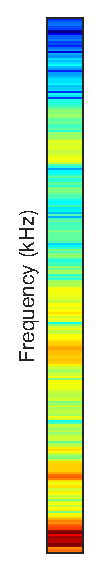
\includegraphics{figs/speech_spectogram_strip.eps}}};
    \node[below = 1mm of spectrogram, text width=2cm, align=center] {Slice of the spectrogram};
    
\end{tikzpicture}